\documentclass[a4paper,10pt]{beamer}
\usepackage[utf8]{inputenc}
\usepackage{color}
\usepackage{colortbl}
\usepackage{xcolor}
\usepackage{caption}
\usepackage{ragged2e}
\usepackage{hyperref}
\renewcommand{\figurename}{Figura}
\usetheme{Warsaw}


% !TEX program = pdflatex


\begin{document}

\begin{frame}
\title{Presentaci\'on Avanzado con Beamer}
\author{Tu nombre ac\'a}
\date{}
\maketitle
\end{frame}

\section[\'Indice]{}
\frame{

\Large{\'Indice}

\tableofcontents

}

\section{Introducci\'on}
\begin{frame}{Introducci\'on}
\justify
Beamer es una clase de LaTeX para la creaci\'on de
presentaciones.

\vspace{0.3cm}
\begin{justify}
Funciona con pdflatex, dvips y LyX. El nombre 
viene del vocablo alem\'an "beamer", un pseudo-anglicismo 
que significa videoproyector. 

\vspace{0.3cm}

En esta presentaci\'on muestro algunas caracter\'isticas avanzadas
de Beamer, entre las much\'isimas que hay, con las que pueden
hacer tu presentaci\'on un poco m\'as din\'amica e interesante.
Hago uso de algunas l\'aminas que hab\'ia creado en para la 
presentaci\'on simple que puedes encontrar \href{https://github.com/FavioVazquez/Presentacion\_Beamer\_Simple}{\color{blue} en este link}
\end{justify}
\end{frame}

\section{Tabla y Ecuaci\'on}
\begin{frame}{Tabla y ecuaci\'on}
  
\begin{enumerate}
 \item Tabla Simple
 
\begin{center}
 \begin{tabular}{l c r } 
	    1 & 2 & 3 %
	    \\ 4 & 5 & 6  %
	    \\ 7 & 8 & 9 \\ %
\end{tabular}
\end{center}

 \item Tres formas de crear ecuaciones

\begin{equation}
E = mc^2
\end{equation}

$$
x^2 + y^2 = z^2
$$

\[ x^n + y^n = z^n \]
\end{enumerate}
\end{frame}

\section{Imagen}
\begin{frame}{Im\'agenes}
\begin{figure}[h]
 \centering 
 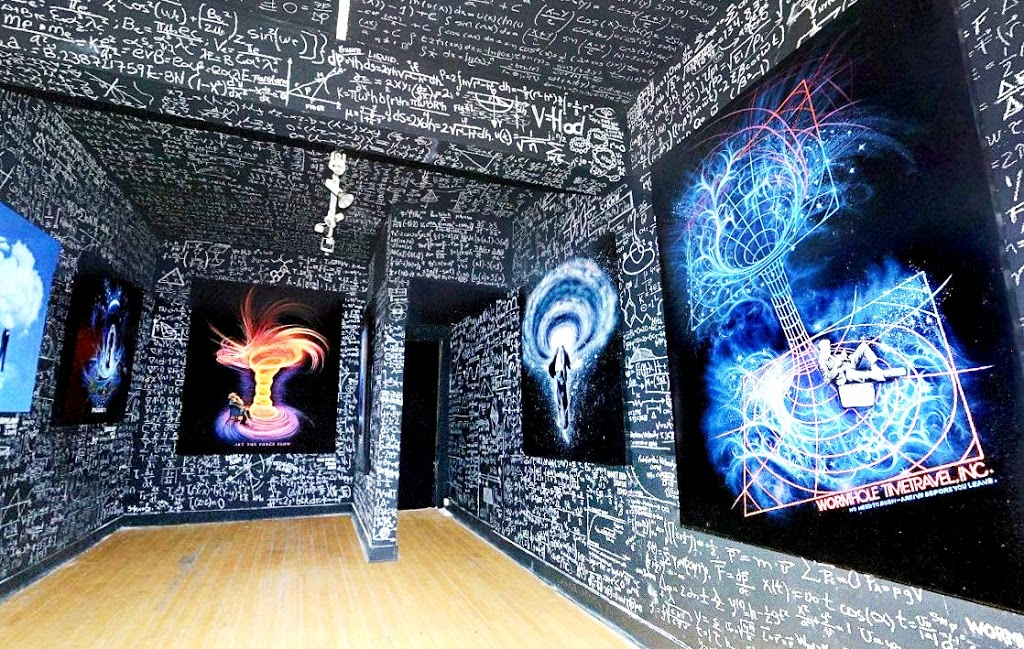
\includegraphics[width=0.8\textwidth]{1}
 \captionsetup[figura]{name=Figura}
 \caption{Bonito Museo}
\end{figure}
\end{frame}

\section{Bloques}
\begin{frame}{Bloques}
 
 \begin{block}{Bloque}
  Esto es un bloque normal
 \end{block}
 
 \vfill
 
 \begin{exampleblock}{Bloque ejemplo}
  Esto es un bloque de ejemplos
 \end{exampleblock}
\end{frame}

\end{document}
